% SHARD-ID: RC-03G-CCM-TENSOR-GRAM
% SHARD-TITLE: CCM in Tensor-Network Terms I: the Weil Form as a Transfer Gram Matrix
% SHARD-SUMMARY: Derives the open-transfer Gram contraction and its metric seams, separating the physical auxiliary, doubled transfer, operator-feature and moment spaces.
% SHARD-SUMMARY: Gives a clock-state purification and a bounded-bond unary-clock MPS, with the exact conjugation and kernel conventions.
% SHARD-KEYWORDS: CCM, Weil form, transfer matrix, Gram matrix, history state, MPS, metric, bond
% SHARD-NOTES: notes/ccm-tensor-network.md
% SHARD-SCRIPTS: scripts/ccm_tensor_network.py

\section{CCM in Tensor-Network Terms I: the Weil Form}
\label{sec:ccm-tn-gram}

The question is how the counts-to-spectrum algorithm acts on the
tensor networks of this notebook. The answer begins with an open
transfer network and a length register. It is essential to say which
space is open. The ladder of \cref{def:ccm-tn-spaces} is
\[
 \TNaux\quad\longrightarrow\quad
 \TNspace\simeq\operatorname{End}(\TNaux)\quad\longrightarrow\quad
 \operatorname{End}(\TNret)\quad\longleftarrow\quad\TNmoment.
\]
For physical auxiliary dimension $D$, the first two dimensions are
$D,D^2$; before retaining modes, vectorised transfer operators have
$D^4$ components. The moment space is a cyclic subspace of this last
space when a suitable representation exists.

\subsection{Closing one ring and comparing two open transfers}

For the local letters of \cref{def:transfer-matrix}, expand the transfer
power and close its two virtual legs:
\[
 \Tr\left(\sum_s A_s\otimes\bar A_s\right)^n
 =\sum_{s_1,\ldots,s_n}\left|\Tr(A_{s_1}\cdots A_{s_n})\right|^2.
\]
This is the usual MPS norm network. The Weil matrix compares different
lengths, so its proposed feature is the \emph{open operator} $E^j$,
not the physical length-$j$ state. Physical states of different lengths
belong to different tensor powers; their direct-sum inner product would
give zero cross terms.

\begin{center}
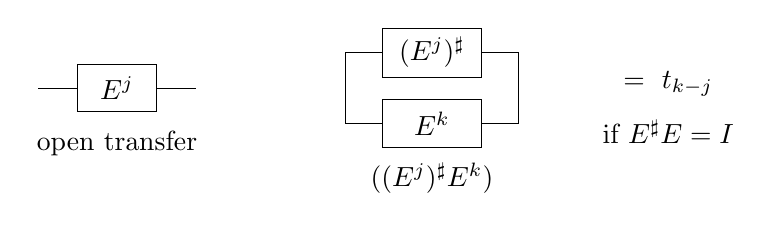
\begin{tikzpicture}[x=1cm,y=1cm,baseline=0]
 \node[draw,minimum width=1cm,minimum height=.6cm] (a) at (0,0) {$E^j$};
 \draw (-1,0)--(a.west); \draw (a.east)--(1,0);
 \node at (0,-.7) {open transfer};
 \node[draw,minimum width=1.25cm,minimum height=.6cm] (b) at (4,.45) {$(E^j)^\sharp$};
 \node[draw,minimum width=1.25cm,minimum height=.6cm] (c) at (4,-.45) {$E^k$};
 \draw (b.west)--(2.9,.45)--(2.9,-.45)--(c.west);
 \draw (b.east)--(5.1,.45)--(5.1,-.45)--(c.east);
 \node at (4,-1.15) {$\Tr((E^j)^\sharp E^k)$};
 \node at (7,.05) {$=\ t_{k-j}$};
 \node at (7,-.55) {if $E^\sharp E=I$};
\end{tikzpicture}
\end{center}
The two connecting wires contract transfer-space indices. Expanding
each $E$ restores the ordinary physical bra/ket layers, hence this
overlap has a further doubling. The adjoint seam contains the metric.

\begin{proposition}[The operator Gram identity and its scope]
\label{prop:ccm-tn-operator-gram}
\claimstatus{prop:ccm-tn-operator-gram}{proved}
If $E^*\TNmetric E=\TNmetric>0$, then for every finite window
\[
 (\TNGram)_{jk}=\Tr((E^j)^\sharp E^k),\qquad
 c^*\TNGram c=\|p_c(E)\|_{\mathrm{HS},G}^2.
\]
In the native metric this holds when $E$ is unitary. Conversely native
Gram equality for \emph{all} nonnegative powers forces native unitarity;
equality on one fixed finite window does not.
\end{proposition}
\begin{proof}
\begin{enumerate}
\item[$\langle1\rangle$1.] The metric identity gives $E^\sharp=E^{-1}$.
Thus $\Tr((E^j)^\sharp E^k)=\Tr E^{k-j}=t_{k-j}$, with the
Hermitian convention for negative lags. Expanding the norm proves the
quadratic identity. Positivity of the operator metric follows by
conjugating by $\TNmetric^{1/2}$, as in \cref{def:ccm-tn-feature}.
\item[$\langle1\rangle$2.] For the converse, all-window Gram equality
gives positive moments of finite rank, since the feature space has
dimension $d^2$. By \cref{thm:weil-positivity-finite}, the eigenvalues
lie in the closed disc. Any interior eigenvalue contributes a strictly
positive Poisson density, which makes every finite monomial Gram
positive definite; this contradicts finite rank for arbitrarily large
windows. Therefore all eigenvalues have modulus one.
\item[$\langle1\rangle$3.] A unitary Schur triangularisation has
$d$ diagonal entries of modulus one. The $j=k=1$ Gram entry gives
$\|E\|_{\mathrm{HS}}^2=d$; the squared absolute values of all
strictly upper triangular entries must consequently be zero. Thus $E$
is unitarily diagonal with unit-modulus eigenvalues.
\item[$\langle1\rangle$4.] On the window $\{0,1\}$, the nonunitary
$X=\left(\begin{smallmatrix}1&1\\0&0\end{smallmatrix}\right)$ has
both native Gram and trace Toeplitz matrix
$\left(\begin{smallmatrix}2&1\\1&2\end{smallmatrix}\right)$.
This disproves the fixed-window converse.
\end{enumerate}
\end{proof}

The required positivity is stronger than positivity of each scalar
ring norm. By the existing Weil theorem it gives a disc bound;
reflection duality supplies the circle, and semisimplicity supplies
an unitarising metric
(\cref{thm:weil-duality-pairing,prop:hp-inner-product-discrete}).
The metric need not descend from a metric on $\TNaux$, and need not
factor over the physical MPS legs. A spectral subtraction alone does
not supply either the retained invariant subspace or those metric seams.

\subsection{A state whose reduced matrix is the Weil form}

\begin{proposition}[Transfer-history purification and an explicit MPS]
\label{prop:ccm-tn-clock-state}
\claimstatus{prop:ccm-tn-clock-state}{proved}
In the metric-unitary setting, the clock marginal of $\TNhistory$
is $\TNGram$, its norm squared is $Kd$, and
\[
 \ker\TNGram=\{c:p_c(E)=0\}.
\]
With $r$ distinct eigenvalues, its unary encoding on $K-1$ clock
qubits has an exact MPS representation of bond at most $2r$,
independent of $K$. Its clock--feature Schmidt rank is $\min(K,r)$.
\end{proposition}
\begin{proof}
\begin{enumerate}
\item[$\langle1\rangle$1.] By \cref{prop:ccm-tn-operator-gram},
$\langle v_j,v_k\rangle=(\TNGram)_{jk}$.
The partial trace of the history in \cref{def:ccm-tn-history} has
entry $\langle\bar v_k,\bar v_j\rangle=\langle v_j,v_k\rangle$.
Its trace is $Kd$. Without the bar on the feature, the marginal is
$(\TNGram)^T$, a real distinction for complex phases.
\item[$\langle1\rangle$2.] The Gram norm identity gives
$c\in\ker\TNGram$ iff $p_c(E)=0$.
\item[$\langle1\rangle$3.] In whitened coordinates write
$\widetilde E=\sum_{a=1}^r z_a P_a$ and set $Z=\operatorname{diag}(z_a)$.
For the un-conjugated history use the virtual matrices
\[
 M_1=\begin{pmatrix}Z&0\\0&0\end{pmatrix},\qquad
 M_0=\begin{pmatrix}0&I\\0&I\end{pmatrix}
\]
on $\mathbb C^r\oplus\mathbb C^r$, left row $(1,\ldots,1;0,\ldots,0)$,
and right endpoint sending either copy of $e_a$ to
$\operatorname{vec}(P_a)$.
Since $M_0M_1=0$, only words $1^j0^{K-1-j}$ survive; their endpoint
is $\sum_a z_a^j\operatorname{vec}(P_a)=v_j$.
Conjugate the matrices and endpoint to obtain $\TNhistory$.
\item[$\langle1\rangle$4.] Evaluation at the $r$ distinct spectral
values is a Vandermonde map, of rank $\min(K,r)$. This is the rank
of the feature family and hence its Schmidt rank.
\end{enumerate}
\end{proof}

The unary construction is an actual tensor network, but its sites
encode length. They are additional clock sites, not a reconstruction
of the original physical chain. The normalised clock density matrix
$\TNGram/(Kd)$ gives an exact entanglement interpretation for this
constructed state. It does not identify the Bost--Connes stationary
state with that density matrix.
